\section{Background}
\label{sec:background}

The converter reads one format and writes another. Most of its design follows from what the
two allow.
This section introduces both Markdown and H5P.

\subsection{Markdown}
\label{sec:bg_markdown}

Markdown is a plain-text markup language: a document is an ordinary text file in which a few
conventions, such as \code{\#} for a heading, \code{*} for emphasis, and a leading \code{-} for a
list item, are interpreted by a renderer.
The original description of the
format~\cite{Gruber:Markdown} was a short, informal document with a reference implementation. It left many cases undefined, such as how list items nest or what happens to an emphasis marker
inside a word.
Each renderer resolved those cases on its own, so the same file rendered
differently from one tool to the next~\cite[Section 1.2]{CommonMark:Spec}.

\paragraph{CommonMark.}
The CommonMark specification~\cite{CommonMark:Spec} removed that ambiguity.
It defines the syntax precisely, with a test suite of several hundred examples. Most current
renderers implement it.
What CommonMark specifies is deliberately small: paragraphs, headings,
emphasis, lists, block quotes, code blocks, links, images, and raw HTML.
Everything else is left to
extensions.

\paragraph{Dialects and Extensions.}
Different platforms and editors thus use their own dialect, i.e., CommonMark
plus their own extensions.
GitHub Flavored Markdown~\cite{GitHub:GFM} adds tables,
strike\-through, and task lists. GitHub also supports footnotes and alerts outside that written
specification~\cite{GitHub:Writing}.
Obsidian~\cite{Obsidian:Links} also adds a link style called wiki links (\code{[[Target]]}), which points at another note by its name instead of
its path.
A third convention comes from the \TeX{} world: formulas between dollar signs, \code{\$x\$}
inline and \code{\$\$x\$\$} for display, which several editors and viewers render as \TeX{} would.
None of these are part of CommonMark, but a converter that accepts real-world documentation
must still accept them.

The converter described in this thesis uses commonmark-java~\cite{CommonMarkJava}, a Java implementation of
CommonMark, together with its extensions that correspond to GitHub Flavored Markdown.
Wiki links and dollar-delimited formulas are handled by two small parsers written for this thesis.
The parser turns Markdown into a tree of nodes:
a document holds block nodes such as paragraphs and lists, and those hold inline nodes such as text
runs, emphasis, and links.
Everything the converter does with a chapter starts from that tree.

\subsection{H5P}
\label{sec:bg_h5p}

H5P is a framework for interactive content.
A piece of content is a
\emph{package}, an \code{.h5p} file that platforms such as Moodle import, render, and edit.
The
package carries the content together with the code libraries the content needs to
run~\cite{H5P:Specification}, so a platform can install these libraries from the package.
Three aspects of H5P matter for this thesis: the structure of a package, the structure
of an Interactive Book, and what may go into a text block.

\begin{figure}[H]
	\centering
	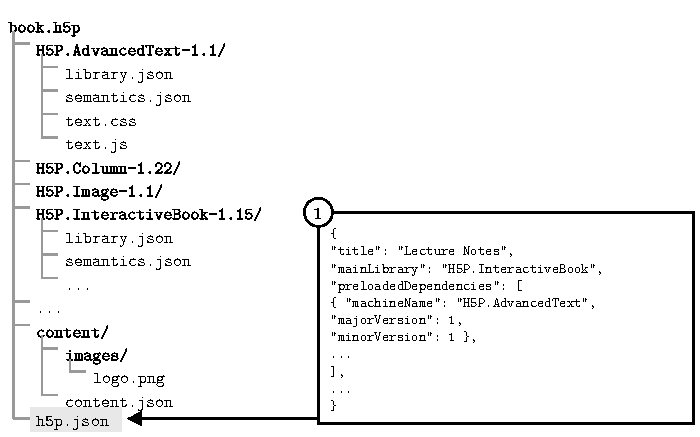
\includegraphics[width=0.9\columnwidth]{figures/package-h5pjson}
	\caption[The layout of a package and its \code{h5p.json}]{\label{fig:package_h5pjson}The layout
		of an \code{.h5p} package and the outline of its
		\code{h5p.json} \circled{1}.}
\end{figure}

\paragraph{Package Structure.}
An \code{.h5p} file is a ZIP archive with a fixed
layout~\cite{H5P:Specification,H5P:FileStructure}, shown in \autoref{fig:package_h5pjson}.
\code{h5p.json} \circled{1} at the root holds the metadata of the content, such as its title and content type, and lists under
\code{preloadedDependencies} every library the content needs~\cite{H5P:PackageDefinition}.

The libraries represent content types and may be bundled as folders named after the library and its version, such as \code{H5P.AdvancedText-1.1}~\cite{H5P:FileStructure}.
Each folder contains a \code{library.json} with its identity and dependencies~\cite{H5P:LibraryDefinition}, a
\code{semantics.json} describing its content model~\cite{H5P:Semantics}, and the
JavaScript and CSS that render it.
A package may, but does not have to, carry the
code of every library it uses~\cite{H5P:Specification}.
On import, the platform installs any libraries it lacks from the package.
If it cannot find them there, the import is refused~\cite{H5P:PhpLibrary}.

\begin{figure}[H]
	\centering
	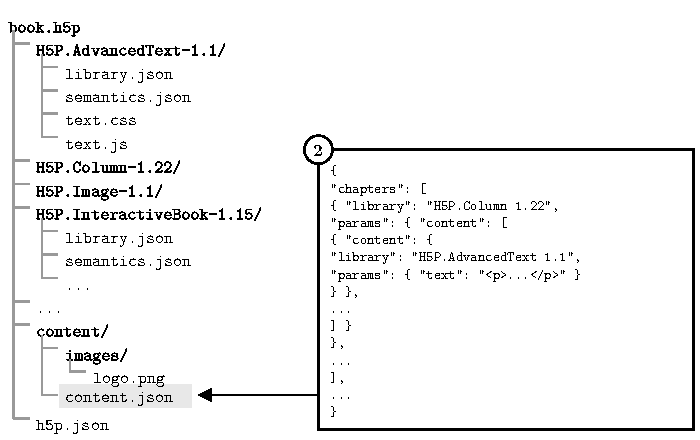
\includegraphics[width=0.9\columnwidth]{figures/package-contentjson}
	\caption[The \code{content.json} of a package]{\label{fig:package_contentjson}The same package
	with its \code{content/content.json} \circled{2} outlined: a list of chapters, each an
	\code{H5P.Column} whose \code{content} list holds the blocks of that chapter, each block
	naming its library and carrying its parameters.}
\end{figure}

The content itself is in \code{content/content.json} \circled{2}, a JSON document in which blocks are nested within other blocks, each providing its content type (\code{library}) and content (\code{params})
(\autoref{fig:package_contentjson}).
Media files referenced from it lie next to it under
\code{content/}, images for instance in \code{content/images}~\cite{H5P:Specification}.

\begin{figure}[H]
	\centering
	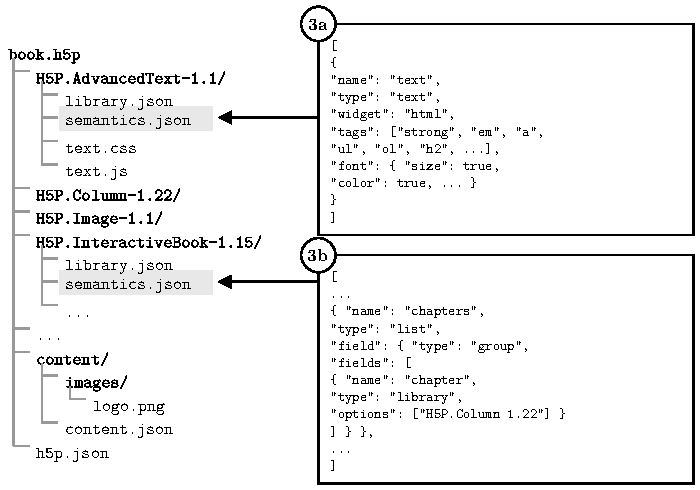
\includegraphics[width=0.9\columnwidth]{figures/package-semantics}
	\caption[The \code{semantics.json} of two libraries]{\label{fig:package_semantics}The same
	package with two \code{semantics.json} files outlined.
	\code{H5P.AdvancedText} \circled{3a} has one field of type \code{text}, with the HTML tags it
	permits and the font properties its editor offers.
	\code{H5P.InteractiveBook} \circled{3b} has a list of chapters, internally represented as \code{H5P.Column} blocks.}
\end{figure}

\code{semantics.json} merits a closer look, because the restrictions
discussed in this thesis stem from it~\cite{H5P:Semantics}.
It is the schema of a content type and describes how the content must be structured and which elements it consists of (\autoref{fig:package_semantics}).
For example, AdvancedText \circled{3a} consists of no more than a text field limited in the set of allowed HTML tags and font styling.
Interactive Book \circled{3b}, by contrast, comprises a list of Column blocks, appropriately called chapters.
For such nesting, a content type must specify the exact versions of the content types it references, tightly coupling the versions of the libraries in a package.

\begin{figure}[H]
	\centering
	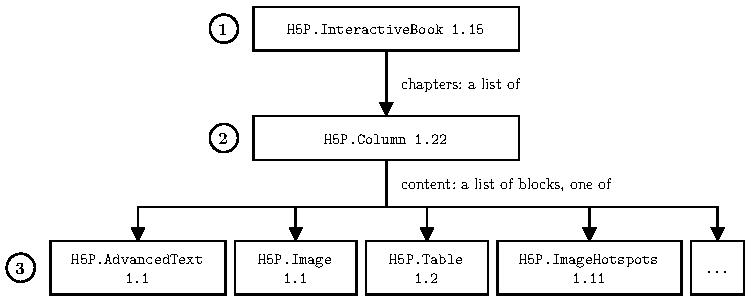
\includegraphics[width=0.9\columnwidth]{figures/book-model}
	\caption[The content model of an Interactive Book]{\label{fig:book_model}The content model of
	an Interactive Book. The book \circled{1} holds a list of chapters, each an \code{H5P.Column}
	\circled{2}, and a column holds a list of blocks \circled{3}, each an instance of one of the
	content types its \code{semantics.json} names.}
\end{figure}

\paragraph{Interactive Book.}
H5P offers many content types, from simple types like AdvancedText and Image to more complicated types such as Course Presentation or Interactive Book that are built from other types.
Interactive Book~\cite{H5P:InteractiveBook} is the one that resembles a multi-chapter document; its viewer shows a table of contents in a sidebar and tracks
reading progress.
In its \code{content.json}, it consists of a list of chapters (\autoref{fig:book_model}),
each chapter being an \code{H5P.Column} \circled{2} and a column being a vertically arranged list of content blocks \circled{3},
each of which is an instance of one of the allowed content types.
The blocks the converter writes are \code{H5P.AdvancedText} for text,
called a \emph{Text block} for brevity, \code{H5P.Image} for images, \code{H5P.Table} for
tables, \code{H5P.Row} with \code{H5P.RowColumn} for a side-by-side layout, and
\code{H5P.SingleChoiceSet} and \code{H5P.MultiChoice} for questions.

\paragraph{Text Blocks.}
A Text block carries one HTML string. This is where the central
constraint of the thesis lies.
Before being shown to the user, a sanitizer runs over it and keeps only the tags the block's \code{semantics.json} permits,
plus a few that are always allowed; a disallowed tag is removed, but its text content is kept.
The remaining HTML tags are further stripped of any illegal CSS styling inside their \code{style} attributes.
Which CSS declarations are allowed is defined in a fixed list specific to each platform (Moodle in this thesis) that the library's
\code{font} declaration in \code{semantics.json} can extend.
Since no stylesheet can be shipped with the content, those
inline styles are the only way to make anything look different from the default.
For now, it is enough to know that \code{img} and \code{table} are among the tags a Text block does not accept: to represent them, the separate Image and Table content types must be used.
